%===============================================================================
% $Id: ifacconf.tex 19 2011-10-27 09:32:13Z jpuente $  
% Template for IFAC meeting papers
% Copyright (c) 2007-2008 International Federation of Automatic Control
%===============================================================================
\documentclass[a4paper]{ifacconf}

\usepackage{graphicx,amsmath,url}      % include this line if your document contains figures
\usepackage[round]{natbib}             % required for bibliography
%===============================================================================https://www.overleaf.com/3833767419zfgrmmhqchmv


% ===============================================================
% Choose the language of the manuscript.
% If in English, choose 
% \def\portugues{0} 
%
% If in Portuguese or Spanish, choose
% \def\portugues{1} 
%
% Note that, if you are writing in Spanish, you need additional 
% adjusts in some parts of the text, which have been put in Portuguese only.
\def\portugues{1} 
% ===============================================================

% If the above line is commented, it is assumed manuscript in English:
\ifx\portugues\undefined
\def\portugues{0}
\fi


\if\portugues0
   \usepackage[english]{babel}
  \else
   \usepackage[spanish,brazil,english]{babel}
\fi

\usepackage[T1]{fontenc}
%\usepackage{inputenc}

\usepackage[utf8]{inputenc}

\usepackage{ae}

\if\portugues1
% =====================================================================
% =====================================================================
% If the manuscript is in Spanish, please change the texts adequatelly.
% You may also add other definitions in this part.
 \newtheorem{teorema}[thm]{{\em Teorema}}{ }
 \newtheorem{lema}[thm]{{\em Lema}}{ }
 \newtheorem{corolario}[thm]{{\em Corolário}}{ }
 \newenvironment{prova}{{\bf Prova.}}{ }
% ===============================================================
\fi

\begin{document}
	
\if\portugues1

% =====================================================================
% =====================================================================
% USE THIS PART IF THE TEXT IS IN PORTUGUES OR SPANISH
% =====================================================================
% If the manuscript is in Spanish, please change the texts adequately.
% =====================================================================
% 
\selectlanguage{brazil}
	
\begin{frontmatter}

\title{Reciclagem Digital: ressignificando o lixo eletrônico}
%--> Ainda podemos pensar num título mais atraente!

\author[1]{Danny A. V. Tonidandel}
\author[1]{Adrielle C. Santana}
\author[1]{Regiane S. S. Ramalho}
\author[2]{Cristiano L. T. F. Silva}

\address[1]{Universidade Federal de Ouro Preto \\ Departamento de Eng. de Controle $\&$ Automação \\ Ouro Preto, MG, Brasil (e-mails: tonidandel@ufop.edu.br, adrielle@ufop.edu.br, regiane@ufop.edu.br)}

\address[2]{Universidade Federal de Ouro Preto\\ Departamento de Eng. de Produção \\ Ouro Preto, MG, Brasil (e-mail: cristiano.silva@ufop.edu.br)}


\selectlanguage{english}
\renewcommand{\abstractname}{{\bf Abstract:~}}
\begin{abstract}                % Abstract of not more than 250 words.
According to the UN, the trash from computer systems as, computers and cellphones, grows at a rate around three times greater than that from the common trash. In just over $60$ years after the creation of computers, with the continouslly growing tax of obsolescence, the amount of trash generated will be converted in a heavy weight for future generations. Between the ways to deal with such a movement, it was created the University Extension Program ``Reciclagem Digital'' that encompassed actions of computers refurbishment and update (\emph{Hospital das Máquinas project}), assembly of computers from electronic junk (\emph{Frankenstein project}) and reuse of damaged electronic components (\emph{Manufatura Reversa project}) from the junk of the University and community. Idealized by professors of the Control $\&$ Automation and Production Engineering Departments of the Federal University of Ouro Preto, the Recicalgem Digital program was one of the success actions to mitigate the environmental impact provoked by the electronic junk. This paper present an experiences report from this educational program, accomplished along the years of $2016$ to $2018$.

\vskip 1mm% não altere esse espaçamento
\selectlanguage{brazil}
{\noindent \bf Resumo}:  Segundo a ONU, o lixo proveniente de sistemas computacionais, como computadores e celulares, cresce a uma taxa cerca de três vezes maior que a do lixo comum. Em pouco mais de $60$ anos após o criação dos computadores, com a taxa de obsolescência cada vez mais precoce, a quantidade de lixo gerada se converterá em pesado fardo para as gerações futuras. Entre as alternativas para se deter tal movimento foi criado o programa de Extensão Universitária ``Reciclagem Digital'' que englobava ações de reforma e atualização de computadores (\emph{Hospital das Máquinas}), montagem de PC's a partir do lixo eletrônico (\emph{Frankenstein}) e aproveitamento de componentes eletrônicos (\emph{Manufatura Reversa}) a partir do lixo da Universidade e comunidade. Idealizado por professores dos cursos de Engenharia de Controle e Automação e Engenharia de Produção da Universidade Federal de Ouro Preto, o ``Reciclagem Digital'' foi uma das ações de sucesso em mitigar o impacto ambiental provocado pelo lixo eletrônico. Este artigo apresenta um relato de experiências desse programa educativo, realizado ao longo dos anos de $2016$ a $2018$.
\end{abstract}

\selectlanguage{english}
\begin{keyword}
Electronic junk, E-waste, Recycling, Urban mining.

\vskip 1mm% não altere esse espaçamento
\selectlanguage{brazil}
{\noindent\it Palavras-chaves:} Lixo eletrônico, E-lixo, Reciclagem, Mineração urbana.
\end{keyword}

\selectlanguage{brazil}

\end{frontmatter}

%===============================================================================
%===============================================================================
%===============================================================================
\section{Introdução: e-lixo não é Lixo!}
É praticamente impossível mensurar o tesouro que está sob nossos pés. E não estamos falando de minério ou outro recurso natural: trata-se do lixo eletrônico, e-lixo ou, da sigla em inglês \textit{E-waste}. Dados oficiais das Nações Unidas, como o observatório global \textit{E-waste} \citep{e-waste}, indicam que mais de $1,5$ milhões de toneladas de lixo eletrônico -- aqueles oriundos de placas de circuito, monitores de computador, celulares e eletrodomésticos -- eram produzidos apenas no Brasil, perdendo para os EUA, que geraram até este ano mais de $6$ milhões de toneladas. No mundo, estima-se que a marca ultrapasse os $50\,mi$ anuais. Apenas $2\%$ do E-lixo brasileiro é reciclado, o que gera um desperdício anual de cerca de $R\$700$ milhões em recursos, e cerca de dez mil empregos que poderiam ser gerados \citep{Salviato}.

A chamada ``Região dos Inconfidentes'' -- Ouro Preto, Mariana e arredores -- é conhecida pela exploração mineral, sobretudo após a maior tragédia ambiental da história, com o rompimento das barragens de mineração a partir de 2016. Neste aspecto, uma mudança de paradigma, que sairia da cultura de ``exploração mineral'' para uma economia ``verde'', baseada no reaproveitamento do lixo eletrônico ou ``mineração urbana'', poderia ser uma alternativa para o futuro da região, iniciando um necessário processo de recuperação dessas localidades, que vêm sendo devastadas continuamente desde o século XVIII. 

No microcosmo das universidades públicas isso também é um problema, e, observando o caso específico da Universidade Federal de Ouro Preto (UFOP), foi proposta uma ação coordenada que buscava atacar o problema em diversas frentes: a manutenção de computadores da comunidade, com objetivo de aumentar o \emph{tempo de vida} dos equipamentos, 
a doação de PC's montados a partir do e-lixo para escolas em situação de vulnerabilidade, e o aproveitamento de componentes eletrônicos para as atividades de ensino e pesquisa da UFOP. Dessas ações surgiu o programa ``Reciclagem Digital''.

\section{Organização, ação e inovação}
A ideia do primeiro projeto surgiu a partir de uma demanda para o laboratório de Instrumentação e Metrologia do Departamento de Engenharia de Controle $\&$ Automação da UFOP. Na ocasião, após uma conversa entre professores e estudantes voluntários, foi combinada uma visita ao \emph{setor de desfazimento} da universidade. Lá observamos uma grande quantidade de peças e sistemas computacionais que estavam com o status de ``obsoletos'' ou ``defeituosos''. A visão era impactante: pilhas e mais pilhas de computadores, monitores, teclados e impressoras, que tinham apenas o lixo como destino (Figura \ref{fig:desfazimento}). Vale ressaltar que o material destinado ao projeto, no setor de desfazimento, consistia daqueles que não mais faziam parte do patrimônio da universidade, já tendo sido destinados ao descarte.

\begin{figure}
	\begin{center}
		\includegraphics[scale=0.7, angle=270]{figuras/desfazimento-UFOP-2016.pdf}    
		\caption{Antigo setor de desfazimento da universidade.} 
		\label{fig:desfazimento}
	\end{center}
\end{figure}

Observamos, porém, que diversos componentes eletrônicos, desde placas de circuitos, monitores e CPU's poderiam ser reaproveitados, não apenas para o laboratório, mas para auxiliar outras pessoas. Alguns dias depois, tendo em mente que um dos objetivos da universidade pública é contribuir para o desenvolvimento material e cultural da sociedade, pensou-se que do ``lixo'' pudessem surgir algumas ações, que foram nomeadas de acordo com seus propósitos: Hospital das Máquinas, Frankenstein e Manufatura Reversa, que integraram o programa \emph{Reciclagem Digital}, cada um coordenado por um professor ou professora.

Após aprovado pela Pró-Reitoria de Extensão da UFOP\cite{proex} com quatro bolsas, no início de 2016, mais dois alunos se juntaram ao projeto de forma voluntária. Após percalços para se encontrar um espaço físico, ferramentas básicas foram adquiridas com recursos próprios dos professores, possibilitando que o programa começasse efetivamente. Como se buscou, desde o início, trabalhar de forma colaborativa e sem uma estrutura hierárquica rígida, uma proposta inédita de organização foi pensada de forma a gerenciar suas atividades. A partir dessa proposta surgiu um novo tipo de infográfico, chamado de ``organograma orbital'' (Figura \ref{fig:organograma}), que ilustra como projetos estariam correlacionados e transmite rapidamente uma visão acerca da organização e grau de envolvimento de cada membro: o programa (``Sol''), no centro , é circundado por projetos (``planetas'') e outros ``corpos celestes'',  que são os recursos humanos. A órbita elíptica mostra, justamente, o grau de aproximação de cada elemento humano e cada projeto dentro de um microcosmo. Essa foi, em essência, a primeira inovação do jovem programa. 

\begin{figure}
	\begin{center}
		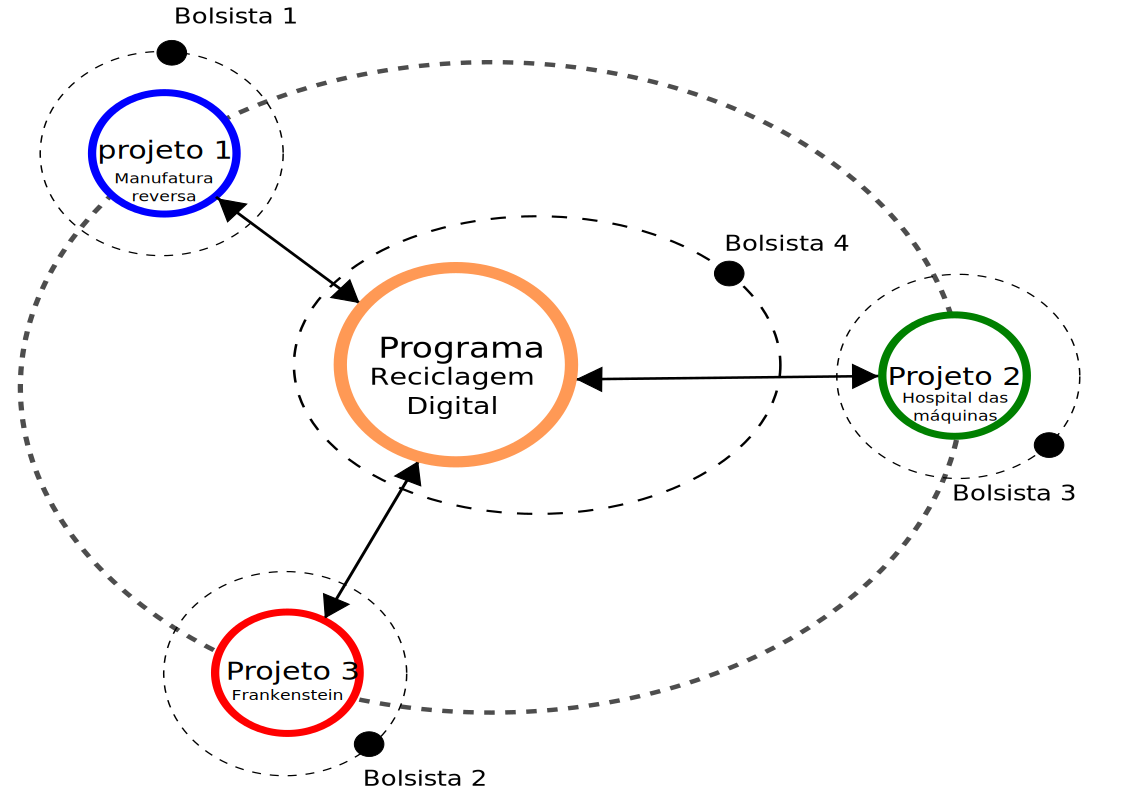
\includegraphics[scale=0.28]{figuras/organograma.pdf}
		\caption{Organograma ``orbital'': um novo tipo de infográfico para projetos colaborativos.} 
		\label{fig:organograma}
	\end{center}
\end{figure}

Outra medida inicial foi realizar um concurso de artes para definir a logomarca que iria ser estampada nos produtos e serviços do programa (Figura \ref{fig:logomarca}) e realizar panfletagem promocional (Figura \ref{fig:panfleto}), de forma a alcançar colaboradores e possíveis beneficiários. Na questão da logomarca, o desafio era transmitir os ideais do programa, bem como fazer uma referência não explícita à atuação da Universidade como elemento transformador da sociedade. Por isso, dadas as regras de utilização da imagem da \cite{ufop2007}, a segunda colocada foi escolhida como marca oficial. 

\begin{figure}
	\begin{center}
		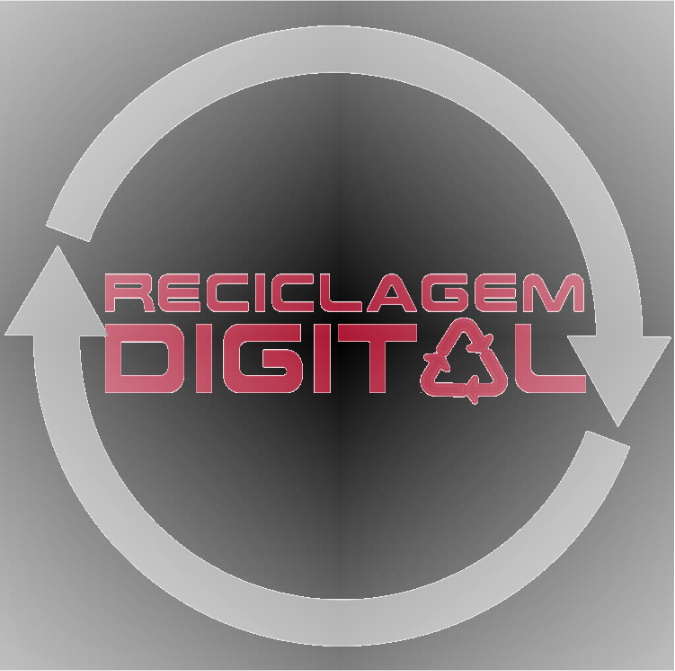
\includegraphics[scale=0.1]{figuras/logo-atual-reciclagem-digital-transparente.pdf}    
		\caption{Logomarca escolhida por um ``concurso de talentos''.} 
		\label{fig:logomarca}
	\end{center}
\end{figure}

\begin{figure}
	\begin{center}
		\includegraphics[scale=0.3]{figuras/panfleto-promocional.pdf}    
		\caption{Um panfleto promocional.} 
		\label{fig:panfleto}
	\end{center}
\end{figure}

\subsection{Hospital das Máquinas}
O objetivo básico do projeto ``Hospital das Máquinas'' era estimular o uso de sistemas computacionais por um período maior de tempo a partir de uma manutenção regular de hardware (futuro “lixo eletrônico”) e atualização de software (futuro “lixo digital”). Isso seria possível com a substituição de componentes defeituosos ou instalação/atualização de sistemas operacionais de fácil manutenção, de preferência software livre e de código aberto. Tal medida visou estender a vida útil das máquinas presentes na comunidade como agente promotora de educação no âmbito socioambiental, além de promover a diminuição da dispersão de material contaminante no meio ambiente. Muitas instituições possuem materiais eletrônicos parados que necessitam apenas de assistência técnica para terem perfeitas condições de uso. Assim, a simplicidade e eficácia consistia em ``colocar para funcionar'' laboratórios de informática, com a instalação de softwares livres, juntamente com um pacote de programas e jogos educativos. Após definidas as instituições a serem beneficiadas, uma visita era agendada, na qual era apresentado o projeto e outras informações. O trabalho seguia, então, dentro da seguinte metodologia:
\begin{itemize}
	\item Se necessário, utilizar peças disponíveis no estoque de ``E-lixo'' do projeto ou setor de descarte;
	\item Instalar de sistema operacional livre e open source (geralmente uma distribuição GNU/Linux);
	\item Instalação de programas e jogos educativos padrão ou sob demanda da instituição atendida.
\end{itemize}

Durante o trabalho, que era normalmente desenvolvido no próprio laboratório da escola, a instituição assinava um documento que comprovasse que os serviços foram prestados pelo projeto.

\subsection{Frankenstein}
Já o projeto ``Frankenstein'' consistia em realizar ações voltadas à doação de computadores – recuperados a partir da área de descarte da UFOP – para instituições de ensino, arte, cultura, religiosas e/ou filantrópicas da região de Ouro Preto e cidades vizinhas. No caso das últimas, seriam beneficiadas desde que exercessem alguma atividade educativa. Eram reaproveitados componentes e peças que viriam a contaminar o meio ambiente por meio de um descarte errôneo ou que continuariam ocupando espaço físico na universidade, além de promover a inclusão digital em instituições onde tais recursos eram escassos. 

A primeira etapa consistia em fazer um levantamento do setor de descarte e, a partir dessa análise, fazer a solicitação de retirada dos equipamentos do setor responsável. Para isto, o setor encaminhava um pedido ao Núcleo de Tecnologia da Informação (NTI) da universidade e, caso liberados, os equipamentos seguiam para a oficina do projeto. Após o levantamento das instituições a serem beneficiadas, os computadores eram montados na medida do possível, realizando-se, em seguida, testes de bancada, troca de peças, formatação e instalação do sistema operacional livre e \emph{open source}, baseado em GNU/Linux. As máquinas eram limpas, embaladas e etiquetadas com a logomarca do Programa, sendo encaminhadas para a instituição beneficiada, finalizando a doação. A última etapa consistia em transportar o lixo não aproveitado para o Projeto de Manufatura Reversa ou para instituições de reciclagem de metais, plástico e eletrônicos.

\subsection{Manufatura Reversa}
O ``Manufatura Reversa'', como o próprio nome indica, consistia em "desmontar para construir", isto é, separar os equipamentos ditos ``obsoletos'' em suas unidades básicas, realizando o movimento inverso ao de uma linha de montagem. Separados, esses componentes (motores de passo, engrenagens, componentes eletrônicos, etc) que poderiam, em tese, ser reaproveitados em outras aplicações, especialmente nas atividades de ensino e pesquisa da universidade. Essa medida visava também auxiliar a comunidade a dar uma destinação útil aos componentes eletrônicos, tais como computadores, TV's, celulares, aparelhos de som, bem como estimular a cultura do reaproveitamento, dado o alto valor agregado nos produtos eletrônicos. Quando era recebida uma solicitação, testes de bancada e triagem dos subcomponentes eram realizados, sendo acondicionados para posterior doação. Dentre todos os projetos, o ``Manufatura Reversa'' tinha também o caráter de projetar componentes sob demanda, o que será visto na seção seguinte.

\section{Resultados}
%
Quando os primeiros equipamentos foram entregues pelo programa, o mesmo já era bem conhecido entre os docentes dos departamentos da unidade. Logo após, o projeto teve a honra da presença do então reitor da UFOP, o prof. Marcone Jamilson de Freitas, na primeira entrega. A cerimônia foi fotografada e, alguns dias depois, uma matéria foi veiculada na página principal da universidade \citep{ufop2016} com grande repercussão na comunidade universitária, como na reportagem de \cite{lamparina}. Em seguida, uma ``chuva'' de solicitações, bem acima da capacidade do programa, começou a acontecer, evidenciando a importância de programas deste tipo para a formação de uma sociedade mais justa. Na ocasião, o reitor da Universidade ressaltou a importância de programas que evidenciam a atuação do servidor público e, especialmente, dos professores em seu papel verdadeiro, o de servirem à sociedade.

\subsection{Hospital das Máquinas}
O projeto ``Hospital das Máquinas'' beneficiou, entre outras, instituições como as Escolas Estaduais Dom Benevides (Figuras \ref{fig:tela7}), Coronel Benjamim Guimarães (Figura \ref{fig:passagem}) e Dom Silvério (Figura \ref{fig:DSilverio}), localizadas na cidade de Mariana-MG. Na última destaca-se a impactante imagem ``antes'' $\times$ ``depois'', em que é possível observar máquinas totalmente inutilizadas por falta de manutenção e reparos. Nestas duas escolas, com a manutenção e assistência de $37$ computadores, sendo $22$ na primeira e $15$ na segunda, estima-se um total de mais de 500 pessoas, entre beneficiados direta ou indiretamente, considerando-se estudantes, professores e funcionários. 

\begin{figure}
	\centering
	\includegraphics[width=7cm]{figuras/cris07.jpg}
	\caption{Teste no laboratório da E. E. Dom Benevides.}
	\label{fig:tela7}
\end{figure}

\begin{figure}
	\begin{center}
		\includegraphics[width=7cm]{figuras/Passagem01.pdf}
		\caption{Laboratório da E. E. Coronel. Benjamin Guimarães.} 
		\label{fig:passagem}
	\end{center}
\end{figure}

\begin{figure}
\begin{center}
\includegraphics[width=8cm]{figuras/dom-silverio-antes-depois.jpg}
\caption{Laboratório de Computação da E. E. Dom Silvério: antes e depois.} 
\label{fig:DSilverio}
\end{center}
\end{figure}

\subsection{Frankenstein}
Durante o projeto \emph{Frankenstein} foi possível realizar a doação de um lote de $11$ computadores a uma instituição de benemerência, que desenvolve ações educativas \citep{ufop2016}, a doação de $3$ máquinas para o movimento dos atingidos por barragens (MAB), uma para a Associação Comunitária de Passagem de Mariana, outra para a Empresa Júnior de Engenharia de Controle e Automação -- \emph{Automic Jr}, além de $10$ máquinas para a organização ``ABCD de combate às drogas'', com sede em Ponte Nova-MG, conforme ilustra a figura \ref{fig:CasaEspirita4}. Os \textit{kits} eram completos, compostos por CPU, mouse, teclado, monitor, cabos de energia e, em alguns casos, um \textit{switch industrial} para possibilitar a montagem de uma rede de comunicação. 

\begin{figure}
 		\centering
 		\includegraphics[width=7cm,angle=0]{figuras/CasaEspirita4.jpg}
 		\caption{Um laboratório montado.}  \label{fig:CasaEspirita4} 
 		\end{figure} 

No total, estima-se que o número de beneficiados direta ou indiretamente ultrapasse as $1000$ pessoas. Em outra atividade, alguns \textit{Totems} foram totalmente recuperados. Um totem é um sistema computacional normalmente utilizado como caixa eletrônico e alguns se encontravam defeituosos, advindos de doações externas.\footnote{Mais especificamente, um totem é um sistema a eventos discretos, mais popularmente conhecido como autômato.} Estes foram recuperados e doados para diversos setores dentro da universidade, tais como a Biblioteca da Escola de Minas, a diretoria da Escola de Minas e o Laboratório de Desenvolvimento de Novas Tecnologias e Prototipagem do DECAT-EM (Figura \ref{fig:totem}). Esses equipamentos estão sendo utilizados em grandes eventos como a Mostra de Profissões, Encontro de Saberes, dentre outros. 

\begin{figure}
	\centering
	\includegraphics[width=5cm]{figuras/totem.jpg}
	\caption{Totem recuperado.}  \label{fig:totem} 
\end{figure}

\subsection{Manufatura Reversa}
A engenharia reversa do projeto ``Manufatura Reversa'' possibilitou a aquisição de componentes e peças
que foram úteis no desenvolvimento de alguns projetos de pesquisa na UFOP, como, por exemplo, um projeto que necessitava de material para a construção de um forno a gás automático em um  trabalho de conclusão de curso realizado por um aluno do curso de Engenharia de Controle $\&$ Automação, como parte de uma pesquisa desenvolvida pelo departamento de Arquitetura e Urbanismo.

Outra articulação com a pesquisa que gerou bons resultados, foi o desenvolvimento de uma solda de termopares por descarga capacitiva a partir de material reciclado, para uso em um laboratório de pequisa da universidade. Dentre todas as solicitações ao projeto, esta foi a que demandou maior esforço de estudo e planejamento por parte do bolsista, envolvendo a área de eletrônica analógica, confecção de placas de circuito impresso, além de propiciar ao estudante o aprofundamento na física inerente ao processo de soldagem.

O projeto incentivou o discente a desenvolver modelos de simulação de circuitos, já que o modelo passado pelo professor da Engenharia Mecânica era baseado em um vídeo oriundo da Internet, que não possuía nenhuma garantia de funcionamento (e, por diversas vezes, não funcionava como deveria). O equipamento consistia em um banco de capacitores ligados em paralelo que, quando ligados a uma carga, descarregam toda a energia em forma de um arco voltaico, fundindo, por resistência, a carga a outro material metálico.  
Adequando-se à ideia central do projeto, o protótipo da solda capacitiva pôde ser construído com materiais reciclados a partir do E-lixo oriundo de placas-mãe e de outros componentes dos computadores de mesa (Figura \ref{fig:capacitores}).

\begin{figure}[h]
	\centering
	\includegraphics[scale=0.2]{figuras/capacitores.pdf}
	\caption{Capacitores podem ser encontrados em placas-mãe de E-lixo.}  \label{fig:capacitores} 
\end{figure}

No equipamento em questão foram utilizados seis capacitores de $4700 \,\mu F$ e $50\,V$, todos eles ligados em paralelo. Para isso, a tensão da fonte, que foi substituída por uma fonte de computador descartado (Figura \ref{fig:fonte}), foi regulada para o máximo de $50\,V$ (em corrente contínua). 

\begin{figure}
	\centering
	\includegraphics[scale=0.1]{figuras/fonte.pdf}
	\caption{A fonte de tensão pôde ser substituída pela fonte de um PC descartado.}  \label{fig:fonte} 
\end{figure}

Uma fontes dessa natureza possui saídas de $12\,V$, $5\,V$ e $3,3\,V$, que podem ser combinadas em série para formar a tensão desejada. Com isso, pôde-se eliminar o uso da ponte retificadora e de uma resistência fixa, presentes no projeto original, pois a fonte de computador já fornece corrente contínua. A resistência variável pode ser substituída por um potenciômetro que, por um \textit{divisor de tensão}, regula a tensão aplicada ao banco de capacitores.

\begin{figure}
	\centering
	\includegraphics[width=8cm]{figuras/simulacao3.png}
	\caption{(acima) Simulação original da solda por descarga capacitiva. (abaixo) Eliminado o uso de ponte retificadora e resistência fixa ao utilizar fonte de PC descartada.}  \label{fig:simulacao3} 
\end{figure}

Ainda no âmbito do projeto Manufatura Reversa, componentes mais simples como dissipadores de calor e engrenagens também foram solicitados e aproveitados por professores do curso de Engenharia Mecânica em suas aulas e projetos. 

\section{Conclusão}
Este artigo buscou realizar um relato de experiências do programa de extensão universitária Reciclagem Digital realizado na UFOP entre os anos de 2016 e 2018. O programa contou com três projetos que, em sua essência, buscaram ressignificar o lixo eletrônico gerado na universidade e na comunidade da região de Ouro Preto-MG e Mariana-MG.

Como resultado, mais de $1000$ pessoas foram beneficiadas direta e indiretamente pelas ações do programa, tanto na comunidade, por meio das instituições atendidas pelos projetos, quanto na universidade, pela redução do lixo eletrônico. Além disso, a disponibilização de materiais para projetos de pesquisa e ativa colaboração da comunidade acadêmica, estimularam o debate sobre melhores formas de gerir os recursos eletrônicos, além de uma maior conscientização sobe a herança que será deixada às gerações futuras. 

Para as alunas e alunos envolvidos, ficou mais do que apenas um aprendizado sobre manutenção de computadores. Eles puderam ver como equipamentos considerados lixo dentro e fora da universidade podem ainda ser muito úteis para quem não tem nada, promovendo a inclusão digital de centenas de pessoas que são e serão atendidas pelas instituições beneficiadas. Além disso, os alunos e beneficiados aprenderam a trabalhar com \textit{Software Livre}, que possui alto desempenho mesmo em máquinas mais velhas, desmistificando-o como algo difícil de se trabalhar.

O programa Reciclagem Digital ressignificou o lixo eletrônico durante a sua vigência na sua pequena região de atuação, porém muito mais é gerado diariamente no país como um todo. Na medida em que o projeto se desenvolveu, foi possível vislumbrar as diversas possibilidades de atuação do programa dada a grande quantidade de lixo eletrônico gerado somente na UFOP. Atualmente, a iniciativa continua por meio de um dos projetos, com alunos voluntários, e ainda muitos equipamento para reciclar e ressignificar.

Espera-se que iniciativas como esta possam servir não só para reduzir o lixo eletrônico, diminuindo seus impactos ambientais, como para promover a inclusão digital daqueles em condições de maior vulnerabilidade social e econômica, mais ``carentes'', redistribuindo melhor tais recursos; inspirar outras pessoas a desenvolverem programas semelhantes em suas instituições ou comunidade; e conscientizar o maior número possível de pessoas sobre o problema do lixo eletrônico no mundo e como ele pode ser ressignificado em nossa sociedade.

\section*{Agradecimentos}
Os autores agradecem à PROEX que acreditou no programa e forneceu as bolsas necessárias aos discentes. O agradecimento se estende à pró-reitoria de administração (PROAD) pela disponibilização de acesso aos setores de desfazimento da UFOP, além dos ex-reitor e vice-reitora da Universidade, prof. Marcone J. F. Souza e profa. Célia Maria F. Nunes. Agradecemos sinceramente aos diversos bolsistas e voluntários que possibilitaram a execução do programa Reciclagem Digital, a citar: Aluizio J. Grecco, Brian A. Fernandes, Ciro Limão, Dauberson Alves Mol, Francisco de Sales Gregorio Neto, Gabriel V. R. Hoffman, Jonisson S. Santos, Heitor A. De Novais, Hamilton Tonidandel Junior, Luciano E. de Almeida, Thiago Vilela Pena, além das dezenas de intusiastas que, de uma forma outra, contribuiram para o sucesso destas ações.
\bibliography{ifacconf}                                                                  

\end{document}
